\section{System Overview}\label{sec:system_overview}

We decided to develop a mobile application, as modern mobile devices already have the capability to interact and collect data from Bluetooth devices like BLE beacons. 
This allowed us to integrate the process of collecting the data, doing classification, and applying the resulting classification model to conduct experiments within the same system.

The application will be developed in C\#\cite{billwagnerDocsGetStarted} with Blazor\cite{BlazorBuildClient} and Razor Pages\cite{tdykstraIntroductionRazorPages2023}.

A primary function of the application is to collect data from the aforementioned beacons. 
As illustrated in figure \ref{fig:ScanAdvertisement}, when the device is running, it will scan for advertisement packets broadcast by the Bluetooth beacons.

\begin{figure}[H]
    \centering
    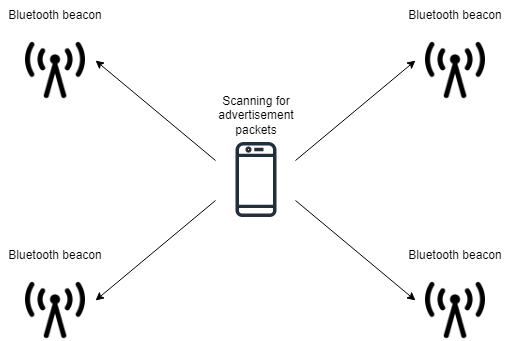
\includegraphics[width=0.5\textwidth]{images/ScanningForAdvertisement.drawio.png}
    \caption{Illustrating a mobile device scanning for Bluetooth beacons.}
    \label{fig:ScanAdvertisement}
\end{figure}

Each beacon broadcasts data, which consists of a unique identifier for the specific beacon and manufacturer-specific information.
A device configured to receive these broadcasts can extract this information and also calculate the received signal strength indicator (RSSI) of the signal.

As outlined in Section \ref{sec:fingerprinting}, fingerprinting involves two stages.
The first stage entails the creation of a map based on the RSSI of the received Bluetooth signal. The second stage involves estimating the unknown location of a Bluetooth receiver.

The application supports the initial stage of fingerprinting - map generation - by collecting broadcast information from the beacons. 
The map creation procedure is demonstrated in Figure \ref{fig:CreateMap}. 
Throughout this operation, a device installed with the application gathers data as it is moved around the room following a particular path.

\begin{figure}[H]
    \centering
    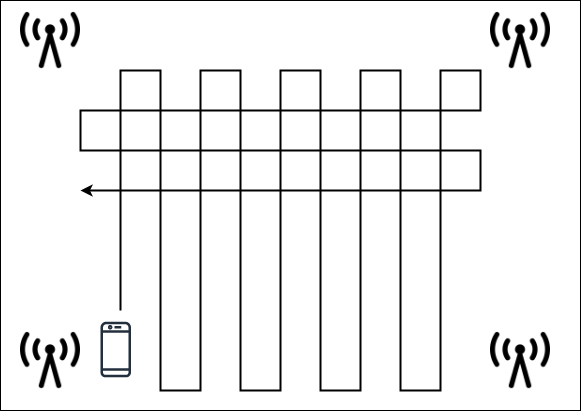
\includegraphics[width=0.5\textwidth]{images/CreateMap.drawio.png}
    \caption{Illustrating a mobile device collecting data from Bluetooth beacons.}
    \label{fig:CreateMap}
\end{figure}

To support the second phase of fingerprinting, we have developed a classification module as part of the application. 
By collecting new data and using the map created during the first phase, the system can classify the position of other devices relative to the room. 
Using the classifier, the application is able to estimate whether a device is either inside or outside the room.

The system diagram in figure \ref{fig:implementation_diagram} illustrates the system architecture and design.
In the following sections, we delve deeper into each phase and component shown in the diagram, offering comprehensive descriptions of crucial aspects of the implementation.
In addition, we present our reasoning behind our chosen methodology.

\begin{figure}[H]
  \centering
  \rotatebox{90}{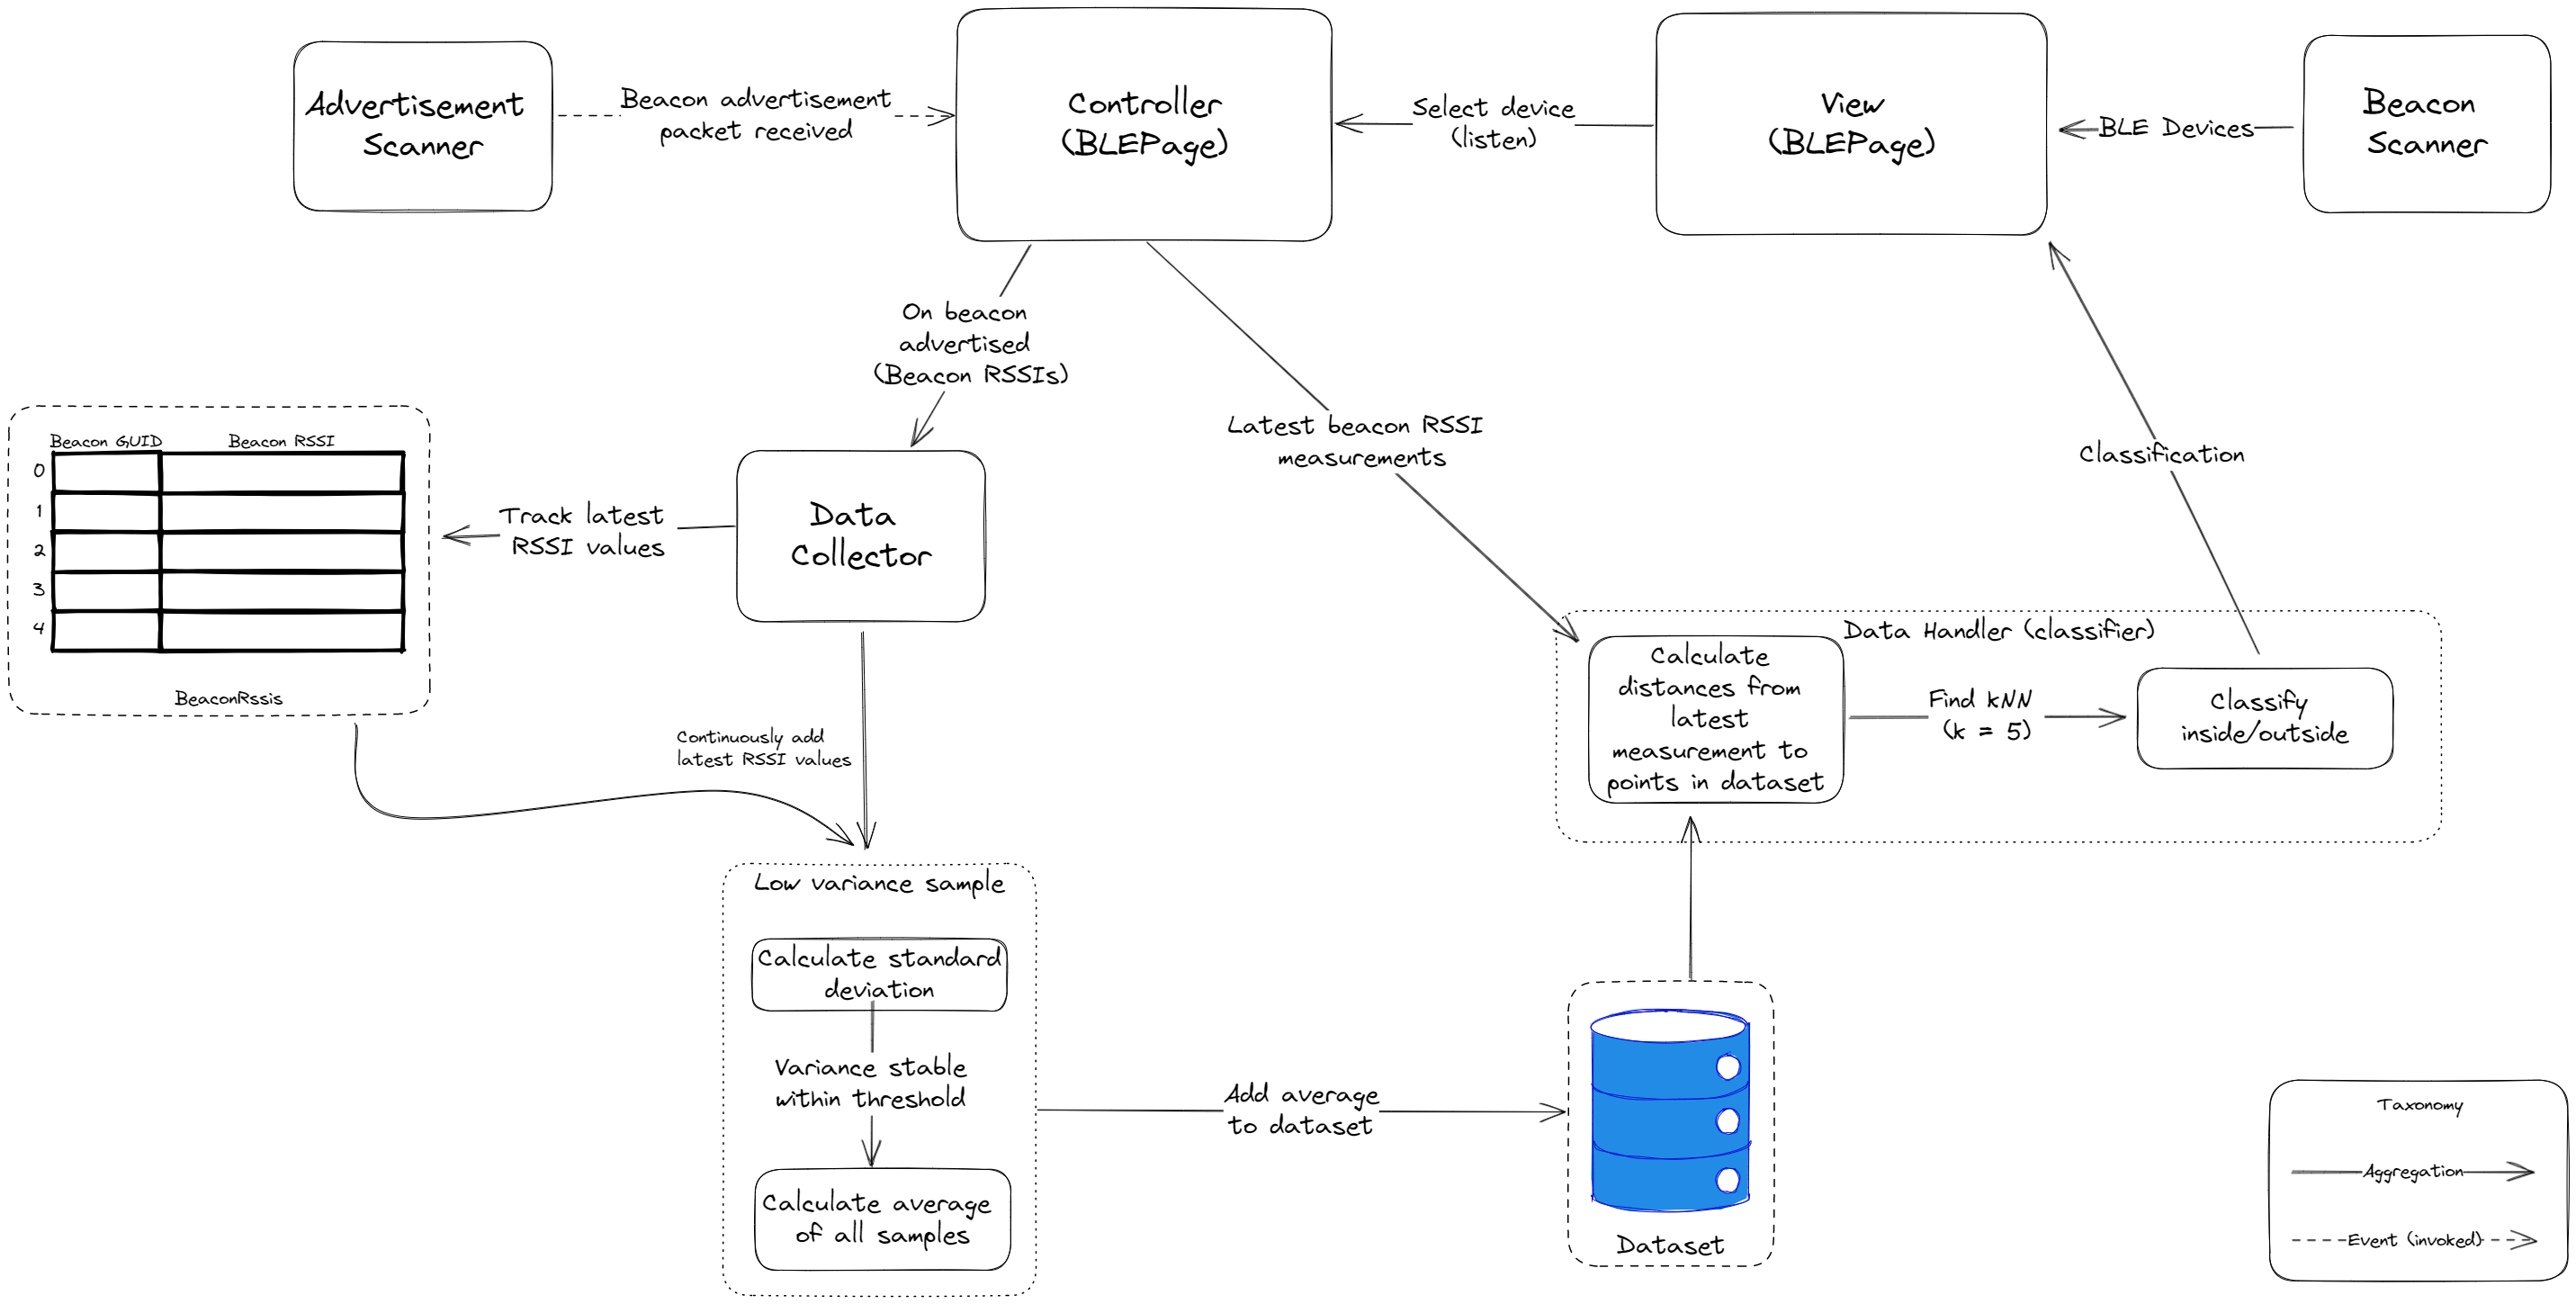
\includegraphics[width=1.75\textwidth]{images/implementation-diagram.png}}
  \caption{Diagram showing the implementation of the system.}
  \label{fig:implementation_diagram}
\end{figure}